\documentclass[a4paper]{article}

\usepackage{graphicx}

\usepackage{latex_packages/FillAFour}
\usepackage{latex_packages/HaskellVerb}

\begin{document}

\title{3802ICT Programming Languages - Assignment 2}


\author{Jesse Schneider}

\maketitle


\begin{abstract}
   This report is targeted at investigating EBNF and parsing for the JavaScript Object
   Notation (JSON) data-interchange format. It includes EBNF definitions, a Haskell
   JSON Data Type, a JSON Lexer and Parser written in Haskell and Validation of the
   parser.
\end{abstract}


\section{Task 1: JSON EBNF}

For this report, we have 2 different sections of EBNF defined:
Lexical syntax and Context-free syntax. Our Lexical EBNF is used to define
Lexical tokens that will be in the parsed content. The Context-free rules 
will define how we combine the Lexical tokens to define rules, in this instance
defining how JSON will be interpreted.

\subsection{Lexical Syntax Rules}

Here is the Lexical EBNF and Railroad Diagrams drawn from those rules,
to display the different Lexical Tokens within JSON:

\subsection*{Whitespace - Spaces, Line Feeds, Carriage Returns, Tabs}

\EBNFInput{EBNF/whitespace.ebnf}

{\centering

   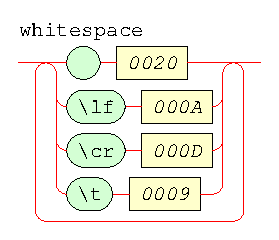
\includegraphics[scale=0.9]{EBNF/whitespace}

}

\subsection*{Digits - All digits from 0 - 9}

\EBNFInput{EBNF/digit.ebnf}

{\centering

   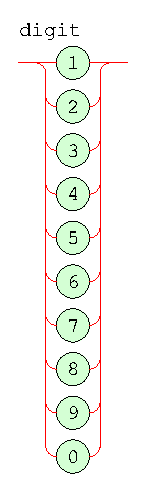
\includegraphics[scale=0.9]{EBNF/digit}

}

\subsection*{Numbers - positive and negative Integer, Decimal, Exponential }

\EBNFInput{EBNF/number.ebnf}

{\centering

   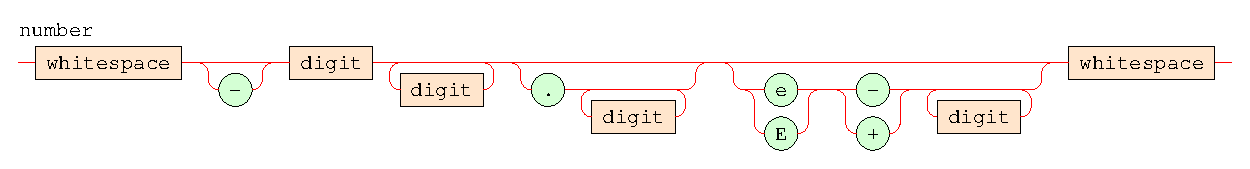
\includegraphics[scale=0.8]{EBNF/number}

}

\subsection*{Strings - A collection of any characters grouped together }

\EBNFInput{EBNF/string.ebnf}

{\centering

   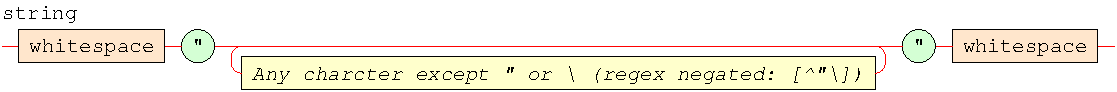
\includegraphics[scale=0.8]{EBNF/string}

}

\subsection{Context-Free Syntax Rules}

Here is the Context-Free EBNF and Railroad Diagrams drawn from those rules,
to demonstrate how the Lexical Tokens can be combined within JSON:

\subsection*{Values - Numbers, Strings, Arrays, Objects, True, False }
\EBNFInput{EBNF/value.ebnf}

{\centering

   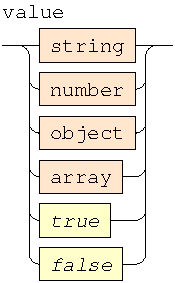
\includegraphics[scale=0.9]{EBNF/value}

}

\subsection*{Arrays - A collection of any Values }

\EBNFInput{EBNF/array.ebnf}

{\centering

   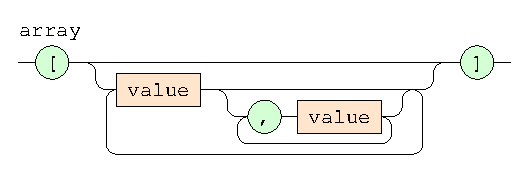
\includegraphics[scale=0.9]{EBNF/array}

}

\subsection*{Objects - A (key:value) type data structure to store any type of Value }
\EBNFInput{EBNF/object.ebnf}

{\centering

   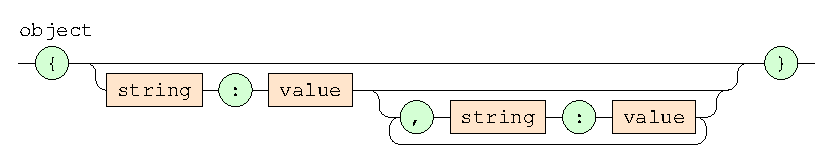
\includegraphics[scale=0.9]{EBNF/object}

}

\newpage


\section{Task 2: Haskell JSON Data Type}

An Algebraic Haskell Data Type has been designed to store JSON as seen here:

Note: Array and Object store repeated JSON objects, so as to contain any other Type of JSON Type.
\input{Code/Parser/Json.lhs}

\newpage

\section{Task 3: Json Lexers + Parsers}

Now that we have a basic idea of what we need for our Lexers and Parsers, its a lot
easier to implement them.

\input{Code/Parser/JsonParser.lhs}

\subsection*{Parsing Test Program}

\input{Code/Parser/JsonP-Test.lhs}

\newpage

\subsection*{Parsing Example}

Here is our input test JSON:
\input{Code/Parser/object.lhs}

\noindent After execution, this is what our Parse Tree looks like:
\input{Code/Parser/output.txt}









\end{document}